\chapter{How He Built a \$200 Million-per-Year Security Company}

The opening image is deliberately simple: cars, a large house, and the obvious question, ``What did this person do to get here?'' In these notes we treat the visible wealth as evidence of an outcome, not as an explanation. The explanation has to be built from the transcript: Edwin Arroyave's early pressure, the home-security business, the transfer into solar, the cash rules that kept risk survivable, and the repeated conversion of desire into deadlines, quotas, and action.

\section{The Visible Puzzle and the Pressure Source}

The interview begins with the surface signal: Lamborghinis, an Aston Martin, and a house in Los Angeles. The narrator immediately turns the signal into an investigation. We are not asked to admire the cars; we are asked to find the mechanism.

The first mechanism is not yet a business model. It is pressure. Edwin says he was born in Colombia, came to the United States at six, and grew up in poverty. Both parents ended up in jail. When his father was put away for a long time, Edwin made a promise that he would take care of the house, and he describes becoming the head of household at fifteen.

That early fact matters because the later language of urgency, necessity, and survival is not decorative. It is the substrate on which the business story rests. If we write the first balance sheet of the story, it is not assets minus liabilities. It is obligation minus preparation:

\begin{equation}
\text{early pressure}
=
\text{family responsibility}
-
\text{ordinary readiness}.
\end{equation}

This is not a literal accounting identity. It is a faithful way to keep the lecture's first turn intact: before there is a company, there is a young person whose tolerance for pressure is being formed.

\section{The Business Base: Security, Solar, and Scale}

The interview then moves quickly from biography to operating facts. Edwin identifies the industry as home security. He has been in it for twenty-five years, began his first business at twenty-one, and is forty-six at the time of the interview. The simple timeline is:

\begin{equation}
46-21=25\text{ years}.
\end{equation}

The revenue claims are given just as directly. The business has generated more than \$600 million over the career, and Edwin says the largest single year will be the current one, at about \$200 million:

\begin{align}
R_{\text{career}} &> \$600{,}000{,}000,\\
R_{\text{year}} &\approx \$200{,}000{,}000.
\end{align}

These should be read as revenue claims, not personal net worth, profit, or valuation. The transcript says the business generated this money; it does not supply margins, ownership percentages, or after-tax proceeds.

Once the numbers are on the table, the interviewer asks the natural scaling question. Many people have ideas; fewer know how to build a nine-figure business. Edwin's answer begins with influence. Good people have options, so they must believe in the leader. The dream has to be large enough that other people's dreams can fit inside it.

We can state the scaling claim as a rough operating dependency:

\begin{equation}
\text{scale}
\;\Longleftarrow\;
\text{recruiting belief}
+
\text{leader's credible dream}
+
\text{first action}.
\end{equation}

The word ``credible'' is important. Edwin does not present dreaming as passive fantasy. He immediately moves to action before resources are fully present.

\subsection{Question \& Answer}

\paragraph{Question.}
How can acting before we have what we need be rational rather than reckless?

\paragraph{Answer.}
The transcript answers with the minivan story. Edwin says that when he started the home-security company, he bought the minivan before he had the people. They used to go door to door in minivans, and he bought the vehicle knowing that the team would come.

The mechanism is not ``spend money blindly.'' The mechanism is commitment under uncertainty. Once money is put behind the future, the desired future stops being optional. Edwin names this a necessity level: a sudden willingness that unlocks ability he did not know he had.

\begin{figure}
\centering
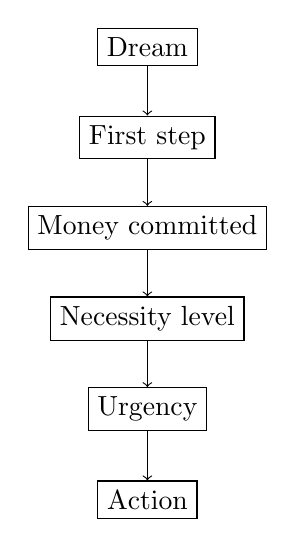
\begin{tikzpicture}[x=1cm,y=1cm]
\node[draw, align=center] (a) at (0,0) {Dream};
\node[draw, align=center] (b) at (0,-1.15) {First step};
\node[draw, align=center] (c) at (0,-2.30) {Money committed};
\node[draw, align=center] (d) at (0,-3.45) {Necessity level};
\node[draw, align=center] (e) at (0,-4.60) {Urgency};
\node[draw, align=center] (f) at (0,-5.75) {Action};
\draw[->] (a) -- (b);
\draw[->] (b) -- (c);
\draw[->] (c) -- (d);
\draw[->] (d) -- (e);
\draw[->] (e) -- (f);
\end{tikzpicture}
\caption{A transcript-grounded reconstruction of Edwin's commitment sequence: the resource is committed before the team is complete, creating necessity and urgency.}
\end{figure}

The important caution is that this is a business psychology claim, not a universal theorem. It works in the transcript because the commitment is tied to a known selling model: door-to-door home-security sales in minivans. The future is uncertain, but the operating path is not imaginary.

\section{Focus First, Diversify Later}

The next question is a classic entrepreneurial fork: should a founder diversify across industries, or focus on one thing? Edwin answers by sequencing the problem. First, become very good at one business. Let that business become the bread and butter. Then diversification becomes a use of earned capacity rather than a substitute for discipline.

The comparison he gives is numerical. It took seventeen years to do \$40 million in one year in security. It took one year to do that in solar:

\begin{align}
R_{\text{security}} &= \$40{,}000{,}000
\quad \text{after }17\text{ years},\\
R_{\text{solar}} &= \$40{,}000{,}000
\quad \text{after }1\text{ year}.
\end{align}

The point is not that every second business can scale seventeen times faster. The point is that an operating discipline can be transferred. Sales structure, urgency, recruiting, standards, and cash-flow discipline were paid for during the first long climb. Solar was not starting from an empty mind.

A cautious way to write the mechanism is:

\begin{equation}
\text{new-business speed}
\approx
\text{market opportunity}
+
\text{transferred operating discipline}.
\end{equation}

The transcript does not isolate the coefficients. It gives the story: become great at one thing, build constant cash flow, and only then take chances in businesses one may not know as well.

\section{The Three-Way Check and the Untouchable Reserve}

The discussion then shifts from revenue to financial advice. Edwin says he did not really have a mentor at the time; one of the great things he did early was split his check three ways. He lived on a third. One third went toward IRS and savings. The other third went into a reserve account that no one could touch.

Let \(I\) denote a check or income event. The transcript-backed allocation can be written as:

\begin{equation}
I
=
\frac{I}{3}_{\text{living}}
+
\frac{I}{3}_{\text{IRS+savings}}
+
\frac{I}{3}_{\text{reserve}}.
\end{equation}

The notation is only a clean reconstruction. It should not be mistaken for tax planning. The transcript does not specify tax rates, account types, investment strategy, or legal structure. The point is behavioral: the reserve account ``did not exist'' for ordinary requests.

\begin{table}
\centering
\begin{tabular}{|c|c|c|}
\hline
Living & IRS + savings & Reserve \\
\hline
Spendable third & Protected obligations & Untouchable buffer \\
\hline
\end{tabular}
\caption{The three-way check split, reconstructed from the interview.}
\end{table}

This rule performs two jobs at once. It prevents lifestyle from absorbing the whole check, and it creates a shock absorber for bad periods. Edwin connects the reserve to a hard claim about life: pain and life are inseparable, so a business builder must expect hard times rather than treat them as exceptions.

\section{A Dream Converted Into a Weekly Sales Requirement}

The most concrete arithmetic in the interview comes from the story of buying his mother a house. Edwin says that at twenty-one he was woken by a roach and decided it would be the last time. At an open house he saw the target in numbers: \$12,000 as a down payment and \$1,400 per month.

He then told his mother the home would be hers in ninety days. That promise converted the dream into a deadline:

\begin{equation}
D=\$12{,}000,
\qquad
M=\$1{,}400/\text{month},
\qquad
T=90\text{ days}.
\end{equation}

The transcript then supplies the operating breakdown. Ninety days is roughly twelve weeks, and Edwin says he needed eight to ten sales for twelve weeks straight:

\begin{align}
90\text{ days} &\approx 12\text{ weeks},\\
S_{\text{week}} &= 8\text{--}10\text{ sales/week}.
\end{align}

\paragraph{Worked target decomposition.}
The point of the calculation is not to infer missing commission data. The transcript does not tell us the commission per sale. The useful derivation is the conversion of a large promise into a repeated weekly action:

\begin{enumerate}
\item State the promise: buy the house for his mother.
\item Put a date on it: \(T=90\) days.
\item Convert time into selling periods: \(90\text{ days}\approx 12\text{ weeks}\).
\item Identify the weekly sales requirement: \(S_{\text{week}}=8\text{--}10\).
\item Use the weekly requirement to govern each day: do not quit at eight or nine o'clock merely because the result has not yet appeared.
\end{enumerate}

The mechanism is clear: the promise changes the meaning of late-day rejection. Without the promise, a weak day can remain a weak day. With the promise, the day is not over until the quota has a chance.

\begin{figure}
\centering
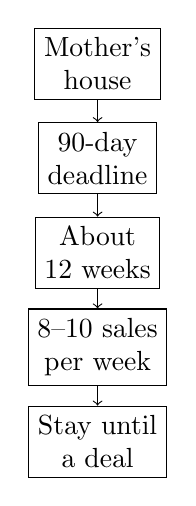
\begin{tikzpicture}[x=1cm,y=1cm]
\node[draw, align=center] (p) at (0,0) {Mother's\\house};
\node[draw, align=center] (d) at (0,-1.20) {90-day\\deadline};
\node[draw, align=center] (w) at (0,-2.40) {About\\12 weeks};
\node[draw, align=center] (s) at (0,-3.60) {8--10 sales\\per week};
\node[draw, align=center] (n) at (0,-4.80) {Stay until\\a deal};
\draw[->] (p) -- (d);
\draw[->] (d) -- (w);
\draw[->] (w) -- (s);
\draw[->] (s) -- (n);
\end{tikzpicture}
\caption{The strongest numerical mechanism in the interview: a dream becomes a dated target, then a weekly sales requirement.}
\end{figure}

This also explains the later confidence claim. Edwin says he stopped looking desperate because he knew that somehow he would get a sale by the end of the day. In the transcript, belief is not floating above behavior. It is produced by repeatedly staying long enough to see a result arrive.

\section{The Abundance Formula}

After the sponsor interruption, the interview returns to money. The question is what separates the middle class from the wealthy. Edwin's answer is framed as a relationship with money. If one is always worried about not having enough, one begins to hoard. If one hoards everything, one never touches or tastes the dream. If the dream is never touched, action never becomes urgent.

The obstacle is a common sequence:

\begin{equation}
\text{wait to have}
\;\Longrightarrow\;
\text{delay action}
\;\Longrightarrow\;
\text{remain stuck}.
\end{equation}

Edwin reverses it. His sequence is:

\begin{equation}
\text{become}
\;\Longrightarrow\;
\text{act}
\;\Longrightarrow\;
\text{have}.
\end{equation}

\subsection{Question \& Answer}

\paragraph{Question.}
Should a person wait until enough money is saved before taking the action that would change the situation?

\paragraph{Answer.}
In Edwin's telling, no. The waiting posture can become a closed loop: save, worry, hoard, postpone, get hit by life, lose the buffer, then start again. The alternative is to become first: cultivate hope, faith, belief, and a sense of worth before the material result exists. Then act before all resources are present.

The key word is not fantasy but breakdown. When action begins, the person receives a blueprint. The large objective must be broken down ``to the ridiculous,'' meaning into units small enough to feel attainable. Once attainable, the target feels realistic; once realistic, action becomes more likely.

The process is best treated as an operating diagram:

\begin{figure}
\centering
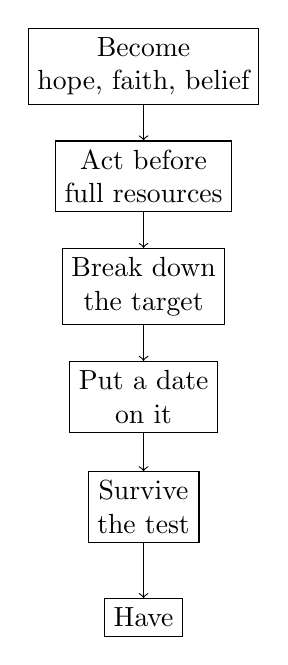
\begin{tikzpicture}[x=1cm,y=1cm]
\node[draw, align=center] (b) at (0,0) {Become\\hope, faith, belief};
\node[draw, align=center] (a) at (0,-1.40) {Act before\\full resources};
\node[draw, align=center] (bp) at (0,-2.80) {Break down\\the target};
\node[draw, align=center] (date) at (0,-4.20) {Put a date\\on it};
\node[draw, align=center] (test) at (0,-5.60) {Survive\\the test};
\node[draw, align=center] (h) at (0,-7.00) {Have};
\draw[->] (b) -- (a);
\draw[->] (a) -- (bp);
\draw[->] (bp) -- (date);
\draw[->] (date) -- (test);
\draw[->] (test) -- (h);
\end{tikzpicture}
\caption{A narrow reconstruction of the abundance formula as the transcript presents it: becoming precedes action, and action produces the blueprint.}
\end{figure}

The hardest part of the formula, Edwin says, is the test near the blessing. The person gets knocked down and must choose whether to revert to excuses or continue forward, focus on what can be controlled, and trust that the right people will appear. The transcript's wording is garbled in this region, but the structure is stable: the test is the point at which the old identity tries to return.

\section{Faith, Happiness, and the Attention Filter}

The last movement of the interview broadens the mechanism. The interviewer asks about people who may not have belief in God or faith in their life. Edwin answers that, whether one likes it or not, one is faith-based. Faith and fear are both projections into a future that has not happened yet:

\begin{equation}
\text{faith}
=
\text{positive projection of the future},
\qquad
\text{fear}
=
\text{negative projection of the future}.
\end{equation}

This should be kept as Edwin's formulation, not as a theorem about psychology. It matters because it links back to action before evidence. A person is already imagining the future; the question is which future governs behavior.

He then distinguishes happiness from pleasure. Exterior factors such as cars, houses, and status brought pleasure, he says, but not stable happiness. Pleasure is a sensation and therefore unstable. It is balanced, in his phrasing, by discomfort and pain. The alternative is living inside out rather than exterior in: gratitude exercises and the ability to turn a negative into a positive.

The final explanatory frame is the reticular activating system. Edwin describes it as part of the subconscious mind, filtering what reaches conscious awareness. We should present this cautiously as his explanatory model. In his version, the filter passes through what has to do with dreams, self-worth, and survival.

\begin{figure}
\centering
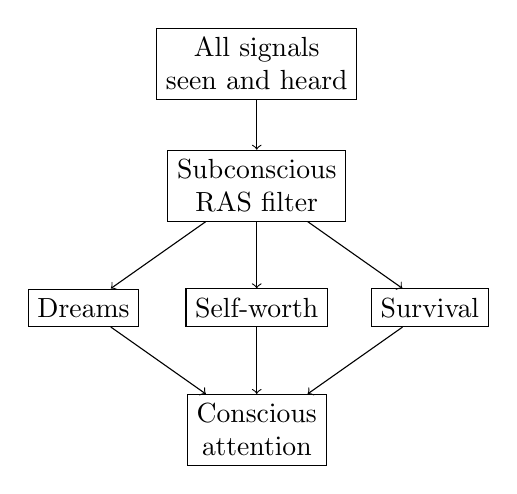
\begin{tikzpicture}[x=1cm,y=1cm]
\node[draw, align=center] (input) at (0,0) {All signals\\seen and heard};
\node[draw, align=center] (filter) at (0,-1.55) {Subconscious\\RAS filter};
\node[draw, align=center] (dream) at (-2.2,-3.10) {Dreams};
\node[draw, align=center] (worth) at (0,-3.10) {Self-worth};
\node[draw, align=center] (survival) at (2.2,-3.10) {Survival};
\node[draw, align=center] (attention) at (0,-4.65) {Conscious\\attention};
\draw[->] (input) -- (filter);
\draw[->] (filter) -- (dream);
\draw[->] (filter) -- (worth);
\draw[->] (filter) -- (survival);
\draw[->] (dream) -- (attention);
\draw[->] (worth) -- (attention);
\draw[->] (survival) -- (attention);
\end{tikzpicture}
\caption{Edwin's attention-filter model, reconstructed from the transcript. It should be read as his framework for opportunity recognition, not as a neuroscience derivation.}
\end{figure}

He then uses that model to reinterpret his own earlier life. At twelve he daydreamed about making \$100,000 by twenty-one. He went to Beverly Hills and imagined ending up there. He had self-worth from early accomplishments, and he needed success for survival because of promises to his parents. In the logic of the interview, those three filters made the opportunity visible when others thought leaving a \$70,000-a-year job was crazy.

\section{Summary}

The chapter's mechanism is not that luxury goods produce ambition, nor that faith alone produces revenue. The transcript gives a more concrete chain. Early pressure creates tolerance for urgency. A focused business creates operating discipline. Influence recruits people. Commitment before complete resources creates necessity. Cash is split so risk does not become fragility. A dream is made useful by converting it into dates and weekly sales. Finally, belief and attention determine which opportunities are even noticed.

The serious quantitative payload is modest but important: twenty-five years from first business to the interview, more than \$600 million in business revenue, a projected \$200 million year, a seventeen-year path to \$40 million in security, a one-year path to the same annual level in solar, a three-way check split, and a 90-day house promise translated into eight to ten sales per week for twelve weeks. These numbers should remain attached to the anecdotes that produced them, because in this interview the arithmetic is not decoration. It is how the dream becomes operational.